\section{Дерево отрезков: модельная задача. Обработка запросов с доказательством времени работы.}

\textbf{Опр} Дерево отрезков (англ. Segment tree) — это структура данных, которая позволяет за асимптотику O(log(n)) реализовать любые операции, определяемые на множестве, на котором данная операция ассоциативна, и существует нейтральный элемент относительно этой операции, то есть на моноиде. Например, суммирование на множестве натуральных чисел, поиск минимума на любом числовом множестве, объединение множеств, поиск наибольшего общего делителя на множестве целых чисел и многочленов.

При этом дополнительно возможно изменение элементов массива: как изменение значения одного элемента, так и изменение элементов на целом подотрезке массива, например разрешается присвоить всем элементам a[l…r] какое-либо значение, либо прибавить ко всем элементам массива какое-либо число. Структура занимает O(n) памяти, а ее построение требует O(n) времени.

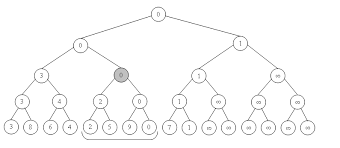
\includegraphics[width = 7cm]{images/60-62_stree}

\textbf{Модельная задача:} Пусть имеется массив размера n: $a_1, a_2, ..., a_n$. К нему поступают 2 вида запросов. На каждый запрос нужно уметь отвечать за O(log(n))
\begin{itemize}
    \item[1] Прибавить к числу на i-й позиции val
    \item[2] Найти сумму на подотрезке [l, r]
\end{itemize}

Окей, в каждом узле дерева будем хранить сумму элементов на контролируемом подотрезке.
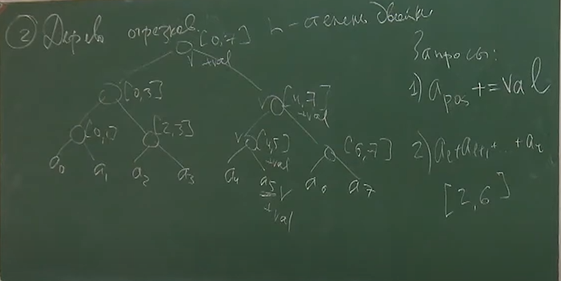
\includegraphics[width = 7cm]{images/60-62_sttask}

Разберемся, как будем отвечать на каждый из запросов.
\begin{itemize}
    \item[1] \textbf{[Прибавить к числу на i-й позиции val]}. Например, нам нужно прибавить val к элементу $a_5$. Тогда значения суммы поменяются только на тех вершинках, которые лежат на пути от корня к листу $a_5$. 
    
    \textit{Асимптотика: высота дерева отрезков log(n). На каждой итерации мы переходим от одного уровня дерева к другому, поэтому время обработки запроса прибавления O(log(n)).}
    \item[2] \textbf{[Найти сумму на подотрезке [l, r]]} Алгоритм обработки этого запроса будет следующий ( рассмотрим для отрезка [1, 3] ):
    \begin{itemize}
    \item Сначала мы стоим в корне, который контролирует весь массив, и смотрим: а правда ли, что интересующий нас отрезок лежит полностью в одном из поддеревьев. В данном случае это верно, правое поддерево нас не интересует, спускаемся в левое([0,3]).
    \item На этом этапе видим, что отрезок не содержится целиком в одном из поддеревьев, поэтому от этого узла нужно пойти в обе веточки. 
    \item Попадая в вершину, контролирующую отрезок [2,3], мы понимаем, что дальше идти не нужно, поскольку отрезок [2,3] полностью содержится в отрезке [1,3]. Дабавляем в сумму значение суммы в узле ([2,3])
    \item Попадая в вершину, контролирующую отрезок [0,1], поступаем аналогично п.1. В левое поддерево нам идти нет смысла, поскольку 0 не входит в отрезок [1,3]. 1 полностью содержится в отрезке [1,3], поэтому добавляем значение суммы из 1. 
\end{itemize}

\textit{Асимптотика: Пусть сначала мы спускались только в одно из поддреревьев. Рассмотрим первый из узлов, в котором нам пришлось спуститься в оба поддерева. Что значит, что мы раздвоились, и отрезок [l,r] лежит частично и слева, и справа? Это значит, что в левом поддереве нам нужно выполнить запрос на суффиксе, а в правом - на префиксе.
}

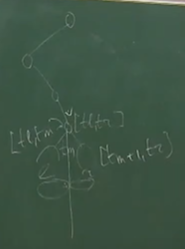
\includegraphics[width = 7cm]{images/60-62_assimpt}

\textit{Давайте поймем, как мы будем себя вести в каждой из веточек. Рассмотрим левую}

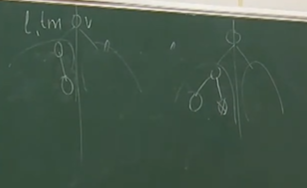
\includegraphics[width = 7cm]{images/60-62_assimpt2}

\textit{Когда идем влево, в правую ветвь левого поддерева мы точно должны спуститься, т.к. запрос происходит на суффиксе. А вот в левую не факт. Но если мы спустились в левую ветвь, это значит, что правая ветвь полностью содержит подотрезок, входящий в искомый, поэтому дальше из правой ветви мы никуда не идем. Аналогично рассуждая для правой ветви, получим, что на каждом уровне дерева может быть посещено не более четырех узлов. Высота дерева log(n). Время работы: O(const *log(n)) = O(log(n)) }

\end{itemize}

\subsection*{Реализация}

\begin{lstlisting}
void SegmentTree::UpdateValue(int index, int newValue) {
	int n = nodes.size() / 2;
	index += n;
	nodes[index].Sum += newValue;
	index = (index - 1) / 2;
	bool end = false;
	while (!end) {
		if (index == 0) end = true;

		nodes[index].Sum = nodes[2 * index+1].Sum +
		nodes[2 *index +2].Sum;
		
		index = (index - 1) / 2;
	}
}
\end{lstlisting}
\begin{lstlisting}
int SegmentTree::getSum( int node, int tl, int tr, int ql, int qr )
{
  if( ql > qr || tl > tr )
    return 0;

  if( tl == ql && tr == qr )
    return nodes[node].Sum;

  int tm = (tl + tr) / 2;
  int leftResult = getSum( 2 * node + 1, tl, tm, ql,min( qr, tm ) );
  int rightResult = getSum( 2 * node + 2, tm + 1, tr,max( tm + 1, ql ), qr );
  return leftResult +  rightResult ;
}
\end{lstlisting}


\section{Дерево отрезков: двоичный спуск, поиск k-го нуля на отрезке массива за O(log n).}


\textbf{Замечание} Используется индексация, начиная с 1

\textbf{Модельная задача:} Пусть в массиве размера n имеются только нули и единицы. К нему поступают два вида запросов:
\begin{itemize}
    \item Поменять элемент на i-й позиции
    \item Найти k-й ноль на подотрезке [l, r]
\end{itemize}

Сведем второй запрос к чуть более простому запросу, когда левая граница отрезка l совпадает с началом массива.

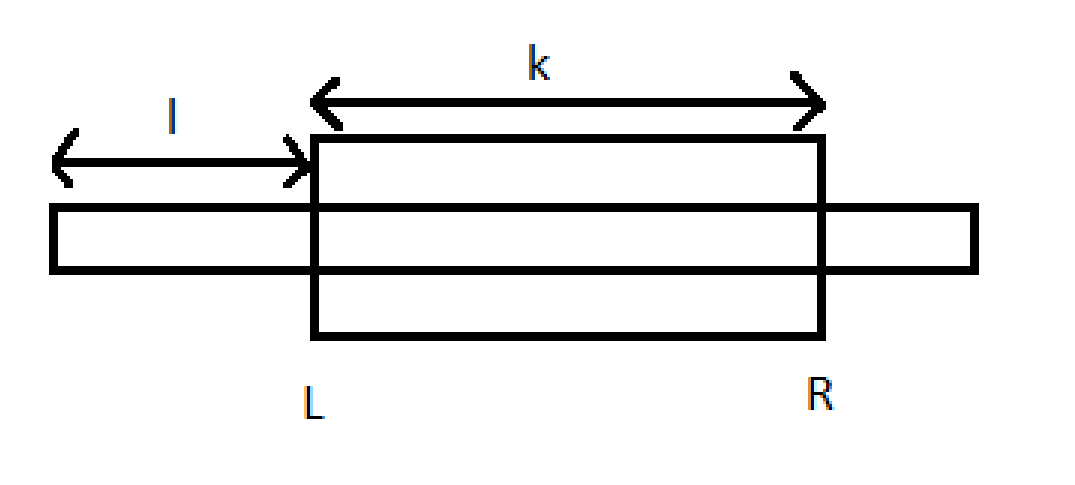
\includegraphics[width=7cm]{images/60-62_2searck}
Тогда поиск k нуля на отрезке [l, r] - то же самое, что и поиск k + l нуля на отрезке [1, r]. Более того, это тоже самое, что найти k + l ноль во всем массиве.

\textbf{Замечание } Для подсчета количества нулей на отрезке будем просто хранить количество нулей на подотрезке в каждой вершине, и считать аналогично подсчету суммы.

Таким образом наша задача упростилась до задачи подсчета k+l-ого нуля на отрезке.
 В каждой вершине будем хранить количество нулей на контролируемом подотрезке.
 
 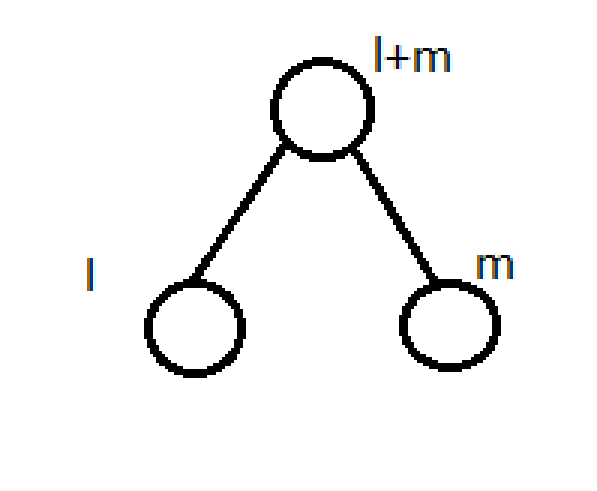
\includegraphics[width=7cm]{images/60-62_seakch2}
 
 Пусть мы находимся в вершине. Всего на подотрезке, ей контролируемой, l + m нулей. 
 \begin{itemize}
    \item[1] Если l+ m < k, то k-ого нуля тут точно нет и не найдется. Иначе:
    \item[2] Если k <=l, то в левом поддереве нулей точно не меньше k, т.е. k-й ноль находится где-то там. Идем в левое поддерево. 
    \item[3]Если же k > l, то k-й ноль находится где-то в правом поддереве, поэтому идем туда, но на подотрезке, контролируемом правым поддеревом, нам нужно найти не k-й ноль, а k-l ноль, поскольку k  нулей уже точно есть на левом подотрезке.
\end{itemize}

Таким образом мы доходим до самого последнего уровня дерева, и находим конкретный индекс


\begin{lstlisting}

    int kth( int index, int l, int r, int key ) {
        if (key > a[index])
            return -1;
        if (l == r)
            return l;
        int middle = (l + r) / 2;
        if (key <= a[index*2] )
            return kth(index * 2, l, middle, key);
        else
            return kth(index * 2 + 1, middle + 1, r, key - a[index * 2]);

}
\end{lstlisting}
\textit{Асимптотика: высота дерева отрезков, состоящего из n элементов, log(n). На каждой итерации мы спускаемся на один уровень вниз, поэтому время работы O(log(n)).}

\section{Дерево отрезков, отложенные операции: прибавление арифметической прогрессии на отрезке, операция push}

\textbf{Модельная задача:} Пусть имеется массив размера n: $a_1, a_2, ..., a_n$. К нему поступают 2 вида запросов.
\begin{itemize}
    \item Прибавить на отрезке арифметическую прогрессию ( т.е. сообщаются 4 индекса l, r, b ,d. $a_l += b$, $a_{l+1} += b+d, ..., a_r += b + (r-l)*d$)
    \item Найти сумму на подотрезке [l, r]
\end{itemize}

\textbf{Идея отложенных операций } Применим следующий трюк: если нам нужно обновить значение подотрезка, то мы отложим эту операцию до востребования. Запомним в соответствующих вершине/блоке, что мы должны в будущем сделать обновление в потомков. Если нам вдруг понадобится значение, лежащее в вершине/блоке, то мы посчитаем его так, как будто мы обновили отрезок, а напоминание о том, что надо сделать со всеми элементами, мы "протолкнем" в потомков.

\textit{Применимо к этой задаче}. В каждой вершине будем хранить пару (b,d) - начальный элемент и разность арифметических прогрессии.

"Проталкивать"  будем следующим образом:

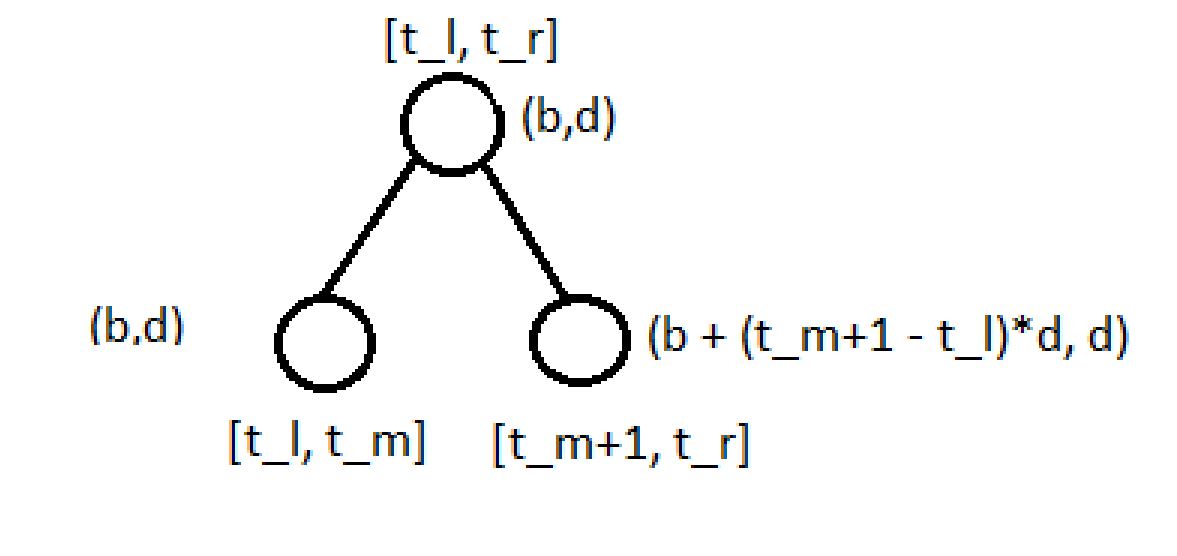
\includegraphics[width=7cm]{images/60-62_fractional1}
В случае, если на отрезке уже была прибавлена какая-то арифметическая прогрессия ($b'$, $d'$), мы просто складываем начальные члены и разности новой и старой арифметической прогрессии

Теперь поймем, как посчитать сумму на отрезке [$t_l, t_r$]. Сумма будет считаться аналогично тому, как мы ее считаем обычно с помощью дерева отрезков, однако теперь к каждому значению суммы в узле будем прибавлять арифметическую прогрессию на подотрезке. Т.е. для значения суммы в каждой вершине:

$n = t_m - t_l + 1$

$S += \frac{2*b + (n-1)d}{2}*n$

Как работать с функцией push (она используется как раз для проталкивания информации в потомков):

\begin{itemize}
    \item Вызывать push надо каждый раз, когда мы обращаемся к вершине, которая могла быть изменена
    \item push-пометки надо не забывать очищать
    \item если мы снимаем push-пометку с единичного элемента, то мы про нее можем забыть
\end{itemize}

\textit{Применимо к этой задаче}. Заходя в вершину на запросе обновления или суммы, мы смотрим, нужно ли что-то протолкнуть в потомков. Если в push-пометке лежит какая-то информация, мы проталкиваем ее вниз и стираем пометку push. Т.е. по-сути мы работаем, как и обычно работали с деревом, просто информацию в вершинах обновляем по мере посещения этих вершин.

\textbf{Пример реализации push для обновления подотрезка}

\begin{lstlisting}
void push(int v, int tl, int tr) {
	if (t[v].push == -1) {
		return;
	}
	if (tl  == tr) {
		t[v].val = t[v].push;
	}
	else {
		t[2 * v].push = t[v].push;
		t[2 * v + 1].push = t[v].push;
	}
	t[v].push = -1;
}
\end{lstlisting}
\textit{Асимптотика отложенных операций: поскольку мы останавливаемся в присвоении, когда текущая вершинка контролирует полностью подотрезок, на котором нужно сделать присваивание, оценка асимптотики будет происходить так же, как и для запроса подсчета на отрезке, т.е. за O(log(n))}